\section{Hopfield Network}

\begin{minipage}[t][][t]{0.75\textwidth}
A Hopfield network \cite{Hopfield, HopfieldCont} has one layer of $N$ neurons and is a fully interconnected recurrent neural network: each neuron is connected to every other neuron.
After initialization of all neurons (the initial input), the network is let to evolve: an output at time $t$ becomes an input at time $t+1$.
Thus to generate a series of outputs, we have to provide only one initial input.
In the course of this dynamical evolution the network should reach a stable state (an attractor), which is a configuration of neuron values that is not changed by subsequent updates of the network.
Networks of this kind are used as models of associative memory.
After initialization the network should evolve to the closest attractor.
\end{minipage}~\hspace{.5em}
\begin{minipage}[t][][c]{0.2\textwidth}
    \centering
    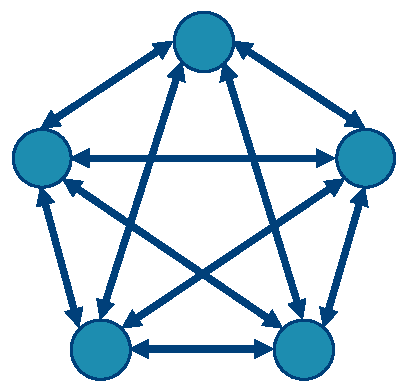
\includegraphics[width=\textwidth]{images/hop.pdf}
\end{minipage}

\kulbox{To answer the questions in this section, you will need the notebook \texttt{hopfield.ipynb} that you can find on toledo, or alternatively using \href{https://colab.research.google.com/github/psanchezML/KUL_ANNDL_ExerciseSessions/blob/main/session2/hopfield.ipynb}{this colab link}.}

%% ===================================================================
%%  THEORETICAL BACKGROUND
%% ===================================================================
\subsection*{Theoretical Background}

\subsubsection*{Energy Function and Dynamics}

The behaviour of a Hopfield network is governed by an \emph{energy function} (also called Lyapunov function).
For binary neurons with states $s_i \in \{-1, +1\}$ and symmetric weights ($w_{ij} = w_{ji}$, $w_{ii}=0$) the energy is
\begin{equation}\label{eq:hop-energy}
    E(\mathbf{s}) \;=\; -\frac{1}{2}\,\mathbf{s}^{\!\top} W\, \mathbf{s} \;-\; \mathbf{b}^{\!\top}\mathbf{s}\,,
\end{equation}
where $W\in\mathbb{R}^{N\times N}$ is the weight matrix and $\mathbf{b}$ is a bias vector.
A fundamental property is that this energy \emph{never increases} during an asynchronous update.
Thus the network always converges to a local minimum of~\eqref{eq:hop-energy}, which corresponds to a stored pattern (or a spurious state).

\begin{insightbox}
The energy landscape can be visualised as a hilly terrain: each stored pattern sits at the bottom of a \textbf{basin of attraction}.
When a (possibly noisy) input is presented, the network ``rolls downhill'' until it settles in the nearest basin, thereby recovering the closest stored pattern.
The deeper and wider the basin, the more robust the recall.
\end{insightbox}

\subsubsection*{Update Rules}

Two update strategies exist:
\begin{itemize}
    \item \textbf{Synchronous}: all neurons are updated simultaneously. Fast but may lead to oscillations in some networks.
    \item \textbf{Asynchronous}: one neuron is updated at a time (randomly selected). Guaranteed energy decrease at every step, hence guaranteed convergence for symmetric weights.
\end{itemize}

% --- TikZ figure: energy landscape schematic ---
\begin{figure}[h]
\centering
\begin{tikzpicture}[scale=0.85]
    \draw[->] (-0.5,0) -- (10,0) node[right] {State space};
    \draw[->] (0,-0.5) -- (0,4.5) node[above] {Energy $E$};
    \draw[thick, blue!60!black, smooth, tension=0.7]
        plot coordinates {(0.5,3.8) (1.5,1.0) (2.5,2.0) (3.5,0.5) (5.0,2.8) (6.5,0.3) (7.5,1.8) (8.5,3.5) (9.5,4.0)};
    \fill[red!70!black] (1.5,1.0) circle (3pt) node[below=4pt] {\footnotesize $\xi^1$};
    \fill[red!70!black] (3.5,0.5) circle (3pt) node[below=4pt] {\footnotesize $\xi^2$};
    \fill[red!70!black] (6.5,0.3) circle (3pt) node[below=4pt] {\footnotesize $\xi^3$};
    \fill[orange!80!black] (2.5,2.0) circle (2.5pt) node[above=3pt] {\footnotesize spurious};
    \draw[-{Stealth}, thick, green!50!black] (4.8,2.6) .. controls (4.2,1.5) .. (3.7,0.7);
    \node[green!50!black] at (4.9,3.1) {\footnotesize noisy input};
    \draw[decorate, decoration={brace, amplitude=6pt, mirror}] (0.7,0) -- (2.2,0)
        node[midway, below=8pt, font=\footnotesize] {Basin 1};
    \draw[decorate, decoration={brace, amplitude=6pt, mirror}] (2.8,0) -- (4.6,0)
        node[midway, below=8pt, font=\footnotesize] {Basin 2};
    \draw[decorate, decoration={brace, amplitude=6pt, mirror}] (5.3,0) -- (7.8,0)
        node[midway, below=8pt, font=\footnotesize] {Basin 3};
\end{tikzpicture}
\caption{Schematic energy landscape of a Hopfield network with three stored patterns $\xi^1,\xi^2,\xi^3$.  A noisy input (green arrow) converges to the nearest basin.  The local maximum between basins~1 and~2 is a spurious attractor.}
\label{fig:energy-landscape}
\end{figure}

\subsubsection*{Storage Capacity}

The \textbf{Hebbian learning rule} stores $T$ patterns of dimension $N$ via the outer-product rule:
\begin{equation}
    W = \frac{1}{T\,N}\sum_{\mu=1}^{T} \boldsymbol\xi^{\mu}\,(\boldsymbol\xi^{\mu})^{\!\top}, \qquad w_{ii}=0.
\end{equation}
A classical result \cite{Hopfield} shows that reliable retrieval is only possible when
\begin{equation}\label{eq:capacity}
    T \;\lesssim\; 0.14\,N\,.
\end{equation}
Beyond this capacity, \textbf{spurious attractors} emerge---stable states that are not stored patterns.
These include mixture states (superpositions of stored patterns) and negations of stored patterns.
The LSSM algorithm (used by MATLAB's \texttt{newhop}) can improve storage beyond this bound by using a more sophisticated weight calculation.

\kulbox{Explore the Hopfield network interactively with the \textbf{Hopfield Basin Explorer} demo app in \texttt{demos/hopfield\_basin\_explorer/}.  It visualises the energy landscape, basins of attraction, and digit reconstruction in 3D.  Run with: \texttt{streamlit run demos/hopfield\_basin\_explorer/app.py}}

%% ===================================================================
%%  EXERCISES
%% ===================================================================
\subsection*{Exercises}
\begin{questions}
    \item Create a Hopfield network with target patterns $[1, 1]$, $[-1, -1]$ and $[1, -1]$ and the corresponding number of neurons.
    Simulate the state evolution for various input vectors (e.g. random points or points of high symmetry) and note down the obtained attractors after a sufficient number of iterations.
    Are the real attractors the same as those used to create the network?
    If not, why do we get these unwanted attractors?
    How many iterations does it typically take to reach the attractor?
    What can you say about the stability of the attractors?

    \item Do the same for a three neuron Hopfield network, this time for the target patterns $[1, 1, 1]$, $[-1, -1, 1]$ and $[1, -1, -1]$.
    Use the analysis tools demonstrated in Exercise~1 (energy landscape, basins, fixed-point classification) to answer the following:
    \begin{itemize}
        \item Are all three target patterns stable fixed points?  If not, which ones are unstable and why?
        \item Visualise the energy landscape slices (at neuron~3 $= -1, 0, +1$).  Where are the energy minima relative to the stored patterns?
        \item Compare the basins of attraction under \textbf{synchronous} vs.\ \textbf{asynchronous} update.  Do the basins differ in shape or size?
        \item Can you find any \textbf{spurious attractors}?  Where do they sit in the 3D state space relative to the stored patterns?
        \item What happens when you start from the origin $[0, 0, 0]$?  Is the outcome deterministic?
    \end{itemize}

    \item Create a higher dimensional Hopfield network which has as attractors the handwritten digits from $0$ to $9$.
    Test the ability of the network to correctly retrieve these patterns when some noisy digits are given as input to the network.
    Try to answer the below questions by playing with these two parameters:
    \begin{itemize}
        \item \texttt{noise\_level} represents the level of noise that will corrupt the digits and is a positive number.
        \item \texttt{num\_iter} is the number of iterations the Hopfield network (having as input the noisy digits) will run.
    \end{itemize}
    Is the Hopfield model always able to reconstruct the noisy digits? If not why?
    What is the influence of the noise on the number of iterations?

    %% --- NEW EXERCISES ---
    \item \textbf{Capacity and Spurious States.}\;
    Systematically increase the number of stored \emph{random} binary patterns for a fixed network size (e.g.\ $N{=}100$).
    For each number of patterns, measure the fraction of patterns that are successfully retrieved after a fixed number of iterations.
    Plot the \emph{retrieval success rate} as a function of the number of stored patterns.
    \begin{itemize}
        \item Identify the experimental capacity threshold and compare it with the theoretical bound $\approx 0.14\,N$ from Eq.~\eqref{eq:capacity}.
        \item Characterise the spurious attractors you find beyond capacity: are they negations of stored patterns, mixture states, or something else?
    \end{itemize}
    Use the \texttt{capacity\_test} and \texttt{find\_spurious\_attractors} methods of the enhanced \texttt{HopfieldNetwork} class.

    \item \textbf{Basins of Attraction Analysis.}\;
    For the 3D Hopfield network from Exercise~2, exhaustively sample the state space (all $2^3 = 8$ binary vertices plus a dense continuous grid in $[-1,1]^3$) and classify each initial state by which attractor it converges to.
    \begin{itemize}
        \item Visualise the basins of attraction using the \texttt{plot\_basins} method.
              Use both the energy landscape (\texttt{plot\_energy\_landscape}) and the basin plot to identify which stored patterns are true attractors and which initial conditions lead to spurious states.
        \item Investigate whether changing from synchronous to asynchronous update affects the basin boundaries.
        \item Discuss the stability of each stored pattern: is every target pattern a genuine attractor?
    \end{itemize}
\end{questions}

%% ===================================================================
%%  MODERN HOPFIELD NETWORKS  (theory only)
%% ===================================================================
\subsection*{Modern Hopfield Networks and the Connection to Self-Attention}

Classical Hopfield networks use a quadratic energy function and binary states, leading to a storage capacity that scales only \emph{linearly} with the network dimension ($\sim 0.14\,N$).
\textbf{Modern Hopfield Networks} \cite{ModernHopfield} replace the quadratic energy with an exponential interaction, dramatically increasing the capacity to \emph{exponential} in the pattern dimension~$d$.

\subsubsection*{Energy and Update Rule}

Given $T$ stored patterns $\boldsymbol\xi^1,\dots,\boldsymbol\xi^T \in \mathbb{R}^d$ and a query (state) $\boldsymbol\xi \in \mathbb{R}^d$, the modern continuous energy is
\begin{equation}\label{eq:modern-energy}
    E(\boldsymbol\xi) \;=\; -\mathrm{lse}\!\bigl(\beta,\, X^{\!\top}\boldsymbol\xi\bigr) \;+\; \tfrac{1}{2}\,\boldsymbol\xi^{\!\top}\boldsymbol\xi \;+\; \text{const},
\end{equation}
where $X = [\boldsymbol\xi^1 \!\mid\! \cdots \!\mid\! \boldsymbol\xi^T]$ stacks the stored patterns as columns, $\mathrm{lse}(\beta, \mathbf{z}) = \beta^{-1}\log\!\bigl(\sum_i e^{\beta z_i}\bigr)$ is the log-sum-exp, and $\beta > 0$ is an inverse temperature.
The corresponding update rule is
\begin{equation}\label{eq:modern-update}
    \boldsymbol\xi^{\mathrm{new}} \;=\; X\,\mathrm{softmax}\!\bigl(\beta\, X^{\!\top}\boldsymbol\xi\bigr).
\end{equation}

\subsubsection*{Equivalence to Transformer Self-Attention}

The update~\eqref{eq:modern-update} is \emph{mathematically equivalent} to one step of Transformer self-attention \cite{Attention}.
The mapping is:

\begin{center}
\renewcommand{\arraystretch}{1.3}
\begin{tabular}{l@{\qquad$\longleftrightarrow$\qquad}l}
    \textbf{Modern Hopfield} & \textbf{Self-Attention} \\
    \hline
    Stored patterns $X$ (Keys) & Key matrix $K$ \\
    State pattern $\boldsymbol\xi$ (Query) & Query vector $Q$ \\
    Pattern projections $X$ (Values) & Value matrix $V$ \\
    $\beta = 1/\sqrt{d_k}$ & Attention scaling \\
    Update: $X\,\mathrm{softmax}(\beta X^{\!\top}\boldsymbol\xi)$ & Attention: $V\,\mathrm{softmax}(Q K^{\!\top}/\sqrt{d_k})$ \\
\end{tabular}
\end{center}

\begin{insightbox}
Transformer self-attention can be interpreted as a \textbf{single retrieval step of a modern Hopfield network}: the query attends to keys (stored patterns) and retrieves a weighted combination of values.
The inverse temperature $\beta$ controls the sharpness of retrieval---large $\beta$ yields one-hot attention (nearest-neighbour lookup), while small $\beta$ yields a soft average.
This unifying view reveals that attention mechanisms in large language models are performing \emph{associative memory retrieval} at every layer.
\end{insightbox}

% --- TikZ figure: Modern Hopfield ↔ Self-Attention ---
\begin{figure}[h]
\centering
\begin{tikzpicture}[
    >=Stealth, node distance=8mm,
    block/.style={draw, rounded corners, minimum width=22mm, minimum height=8mm, align=center, font=\small},
    op/.style={draw, circle, inner sep=1.5pt, font=\footnotesize},
]
    % Modern Hopfield side
    \node[font=\bfseries] (mh_title) {Modern Hopfield};
    \node[block, below=5mm of mh_title] (xi) {Query $\boldsymbol\xi$};
    \node[block, left=12mm of xi] (X) {Stored $X$};
    \node[op, below=8mm of xi] (dot1) {$\cdot$};
    \node[block, below=8mm of dot1] (sm1) {$\mathrm{softmax}(\beta\;\cdot)$};
    \node[op, below=8mm of sm1] (dot2) {$\times$};
    \node[block, below=8mm of dot2] (out1) {$\boldsymbol\xi^{\mathrm{new}}$};

    \draw[->] (xi) -- (dot1);
    \draw[->] (X) |- (dot1);
    \draw[->] (dot1) -- node[right, font=\scriptsize]{$X^{\!\top}\boldsymbol\xi$} (sm1);
    \draw[->] (sm1) -- (dot2);
    \draw[->] (X) |- (dot2);
    \draw[->] (dot2) -- (out1);

    % Self-Attention side
    \node[font=\bfseries, right=40mm of mh_title] (sa_title) {Self-Attention};
    \node[block, below=5mm of sa_title] (Q) {Query $Q$};
    \node[block, left=12mm of Q] (K) {Keys $K$};
    \node[op, below=8mm of Q] (dot3) {$\cdot$};
    \node[block, below=8mm of dot3] (sm2) {$\mathrm{softmax}(\cdot/\!\sqrt{d_k})$};
    \node[op, below=8mm of sm2] (dot4) {$\times$};
    \node[block, right=12mm of K] (V) at (K -| sa_title) {Values $V$};
    \node[block, below=8mm of dot4] (out2) {Attention output};

    \draw[->] (Q) -- (dot3);
    \draw[->] (K) |- (dot3);
    \draw[->] (dot3) -- node[right, font=\scriptsize]{$QK^{\!\top}$} (sm2);
    \draw[->] (sm2) -- (dot4);
    \draw[->] (V) |- (dot4);
    \draw[->] (dot4) -- (out2);

    % Equivalence arrow
    \draw[<->, ultra thick, red!60!black, dashed] ([xshift=6mm]sm1.east) -- ([xshift=-6mm]sm2.west) node[midway, above, font=\small\bfseries, red!60!black] {$\equiv$};
\end{tikzpicture}
\caption{The Modern Hopfield update (left) is structurally identical to Transformer self-attention (right).  Stored patterns play the role of Keys, the query state maps to the Query, and the retrieved output corresponds to the attention-weighted Values.}
\label{fig:modern-hopfield-attention}
\end{figure}

\subsubsection*{Exponential Storage Capacity}

While classical Hopfield networks can store at most $\sim 0.14\,N$ patterns, modern Hopfield networks achieve a capacity that is \emph{exponential} in the pattern dimension:
\begin{equation}
    T_{\max} \;\sim\; \exp\!\bigl(\alpha\, d\bigr), \qquad \alpha > 0.
\end{equation}
This exponential scaling is enabled by the log-sum-exp energy, which creates much sharper separation between stored patterns in the energy landscape.
Intuitively, the softmax creates a ``winner-take-all'' competition among stored patterns, allowing far more patterns to coexist without interference.

\kulbox{Explore the connection between Modern Hopfield Networks and self-attention with the interactive demo in \texttt{demos/modern\_hopfield\_attention/}. It lets you compare classical vs.\ modern retrieval, adjust the temperature $\beta$, and visualise how attention maps sharpen.
Run with: \texttt{streamlit run demos/modern\_hopfield\_attention/app.py}}
